\section{Best practices: beautiful code, GitHub, and notebooks}
\label{sec:practices}


This section gives a brief explanation of ``computational hygiene'': how to structure your code such that you can understand it later, the importance of naming and documentation, the use of versioning and online repositories such as GitHub, and the use of literate programming (such as through the use of RMarkdown or Jupyter notebooks) to explain, share and publish code.

Coding is more than learning the basic rules and creating a message. If you want use the code to communicate ideas and to work with peers you have to take care of many content and shape details in order to guaranty the comprehension and reproducibility of the scripts. It even applies to the code you write for ``private use'' because it is highly likely that you forget your original thoughts from one day to another, or that you later realize that you need to share it with someone else to ask for help. Thus instead of writing personal, hidden and \textit{illiterate} code without adopting any social conventions, you should dedicate some extra effort to have your scripts easy and ready to share.

The first step of the computational hygiene is within the very code. Every time you create an object, a variable or a function you have to take many apparently unimportant decisions when giving a name, separating words, lines or blocks, and including comments. These decisions are personal but mostly should depend on social conventions in order to be useful. As you may imagine, there are many of these conventions for general programming and specially for specific languages. Just to mention some, you can find an ``official'' style guide for Python\footnote{https://www.python.org/dev/peps/pep-0008/}  or Google's R style guide\footnote{https://google.github.io/styleguide/Rguide.html}. Some of these guides are extensive (they cover every detail) and some are more general or abstract. You do not have to see them as a ``bible'' that needs to be strictly adhered to in each and every situation, but they offer very good guidance for best practices. In fact, even when you find them useful it is true that you will probably learn more of these practices from reading good examples and specially from interacting with a specific community and its rules.

We will mention some general guidelines that apply for both R and Python. If it is the first time you are into the world of code you will find these advices useful,  but if you are a more advanced learner you will probably get more specific knowledge in more detailed sources for each language and community.

In the case of naming we encourage you to use meaningful names or standard abbreviations to objects, using lower-case or mixed-case (remember it's case-sensitive!), avoiding special characters and operators (such as \&, @ or \%), and not exceeding 32 characters. You normally begin with a letter\footnote{An exception are so-called private identifiers -- identifiers that are not supposed to be direclty addressed. They conventionally begin with an underscore.} (an upper-case when defining a class), followed by other letter or numbers, and using underscores to separate the words if it is necessary (i.e. \texttt{data\_2020} or \texttt{Filter\_Text}). Some suggest that variable names should be nouns and function names should be verbs, which seems logical if you think of the nature of these objects. 

When writing the code, please take also into consideration the white spaces and indentations (remember 2 spaces for R and 4 for Python!), because you should use them to give proper structure to the code by creating the block statements (in the case of R also pay attention to the use of curly braces\footnote{The convention is that the opening curly begins after some code and is always followed by a new line; and the closing curly is in its own line except if there are more instructions in the block}). Do not write very long lines (more than 80 characters) to help your code fit the screen and avoid lateral scrolling. Good separation of words, lines and blocks will make your script more readable!

Now, if you want to make your code highly understandable and shareable, you have to include \textit{documentation}.
This is probably a very basic dimension of coding but unfortunately some authors forget to include some few words of what they have done in their scripts, making your journey (and sometimes their own!) more difficult.
An essential good practice in coding is to include enough information that clarify your code when it is not clear by itself.
You can do this in different ways (even by writing a separate codebook), but the most natural and straightforward manner is to include some  \textit{comments} in the code.
This comments should be included both at the beginning of the script to give an overview or introduction to the code;
and within the script (in independent lines or at the the end of a line) to give specific orientations.

R and Python use the hash sign \texttt{\#} to create these comments. Notice that the comment will begin always after the hash, so this part will not be executed when compiling. If the first character in your line is  a \texttt{\#} all the text included will be considered as a comment; but if you have already written some code in a line and include a \texttt{\#} after the code, the initial code will be executed and you will always see the comment by its side. You will normally combine these two ways of documenting your script.
As a rule of thumb, insert a comment if the code itself is not obvious,
and explain the choices and intentions of the code.
So, if a line says \verb|df = df - 1|, a comment like \emph{Decrease df by one} is not very useful (as that is obvious from the code), but a comment like \emph{Remove one degree of freedom since we esimated the mean} does help, as it makes it clear why we are subtracting one from the \verb|df| object.

Additionally, Python and R encorage the use of so-called \fn{docstrings}:
In Python, place a string surrounded by triple quotation marks at the start of a function; in R, place a commend \verb|#'| right above the function.
\footnote{For more information, see \url{https://www.python.org/dev/peps/pep-0257/\#what-is-a-docstring} and \url{https://cran.r-project.org/web/packages/roxygen2/vignettes/roxygen2.html},respectively}
In this documentation, you can explain what the function does and what parameters it requires. 
The neat thing is that if properly used, docstrings are automatically displayed in help functions and automatically generated documentation.

Another way to make your code more beautiful and, crucially, easier to re-use by others and/or your future self is to make your code as generic as possible. For instance, imagine you need to calculate the sum of the length of two texts, ``Good morning!'' and ``Goodbye!''. You could just write |r = 13 + 8|. But what if the strings change in the future? And how to remember what |13 + 8| was supposed to mean? Instead of using such \emph{hardcoded} values, you can therefore better write |r = len("Good morning!") + len("Goodbye")| (in Python, in R replace \fn{len} by \fn{nchar}. But the strings themselves are still hardcoded, so you can better create these strings and assign them the names |s1| and |s2| first, and then just calculate |r = len(s1) + len(s2)|. In practice, these types of generalisation often involve the uses of functions (\refsec{functions}) and loops (\refsec{loops}). So, don't use hard-coded values or ``magic numbers'': \verb+circumference=6.28*r+ is much less clear than \verb+PI=3.14; circumference=2*PI*r+.

Moreover, you must be aware that your code is \textit{dynamic} and it will normally evolve over time. For example, you may have different files (.py or .R) containing different versions of your script, though this is normally inefficient and chaotic. In order to have a more powerful control of versions and to track changes, coders usually use online repositories to host their scripts for private use and especially to share them. And there are many of these sites, but we could fairly say that Github\footnote{https://github.com/} is the most known and preferred by data scientists (Figure~\ref{fig:github} shows the repository we used to write this book together).

\begin{figure}
\centering
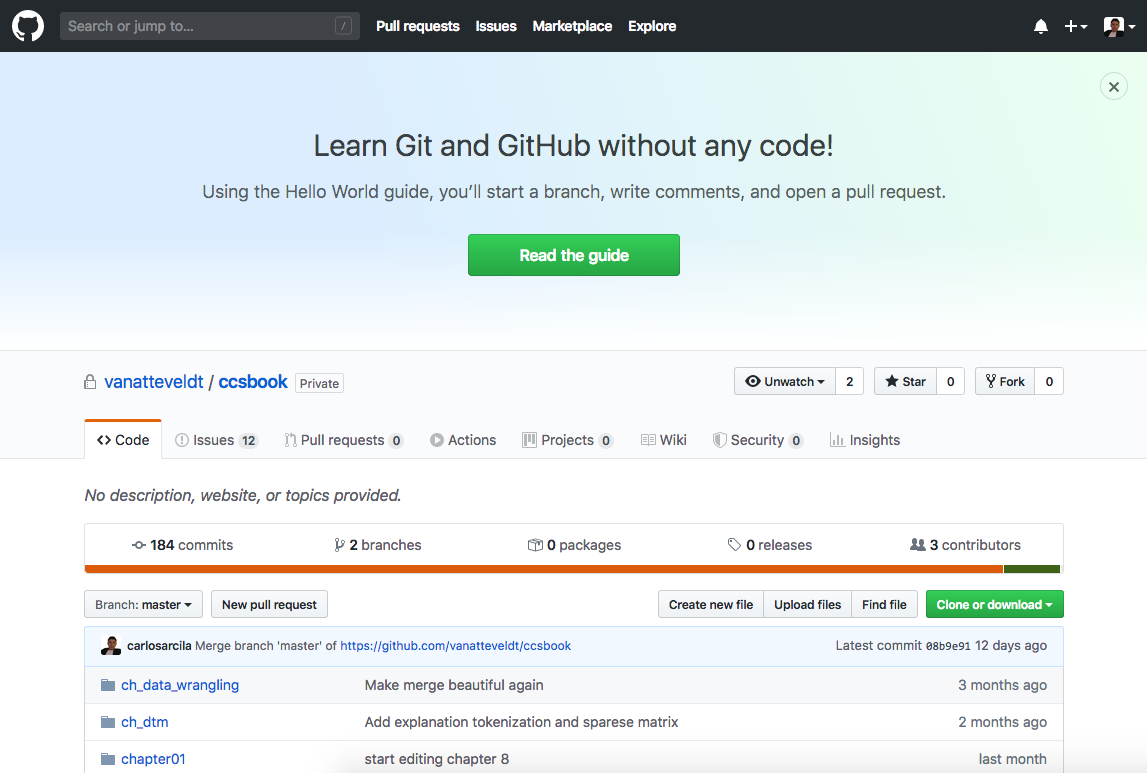
\includegraphics[width=0.9\linewidth]{figures/ch04_github}
\caption{The online repository GitHub}
\label{fig:github}
\end{figure}
 
Once you upload (or \textit{commit}) your code to GitHub you can have access to it from anywhere and will be able to track the historical changes, which in practice will allow you to have multiple versions in the very same place. You will decide if you keep the code public or private, and who to invite to edit the repository. When working collaboratively you will feel like editing a \textit{wiki} of code, while having a \textit{webpage} for your project and a \textit{net of friends} (followers), similarly to a social media. You can work locally or even from a web interface, and then synchronize the changes. When you allow colleagues to download (or \textit{clone}) your repository you are then making a good contribution to the community of developers and you can also monitor your impact. In addition to code, you can also upload other kind of files, including notebooks, and organize them in folders, just as you have it on your computer.

One extended good practice when sharing code is the use of \textit{literate programming}, which is an elegant, practical and pedagogic way to document and execute the base code. We have already mentioned in this section the importance of including documentation within your code (i.e. using the \texttt{\#} sign and docstrings), but you also have the opportunity to extend this documentation (with formatted texts, images and even equations!) and put everything together to present in a logical structure all the necessary to understand the code and to run the executable lines step by step. 

There are different approaches to implement this literate programming in web and local environments, but the standard in R and Python is the use of \textit{notebooks}. In a notebook you can alternate a text processor with a executable cell to include formatted contents and blocks of code, respectively. By doing this you can include complete documentation of your scripts, and even more important you can execute each cell one step at a time (loading the results in RAM memory while the notebook is open). This last point allows you to avoid the risks of executing the whole script at once, and also to have more control of the intermediate outputs produced in your code. Once you get used to notebooks, you will probably won't want to write code for data analysis in a basic editor again!

The usual tool in R is the \textit{R Markdown Notebooks} and in Python the Jupyter Notebooks (see figure~\ref{fig:notebooks}), but in practice you can also deploy Python in Markdown and R in Jupyter. Both tools can help you with similar task to organize your script, though their internal technical procedures are quite different. We have chosen Jupyter to develop the examples of this book because it is a web-based interactive tool. Moreover, there several services such as Google Colab\footnote{https://colab.research.google.com} (Figure~\ref{fig:colab}), that allows you remotely run these notebooks online without installing anything in your computer, making the code highly reproducible.

\begin{figure}
\centering
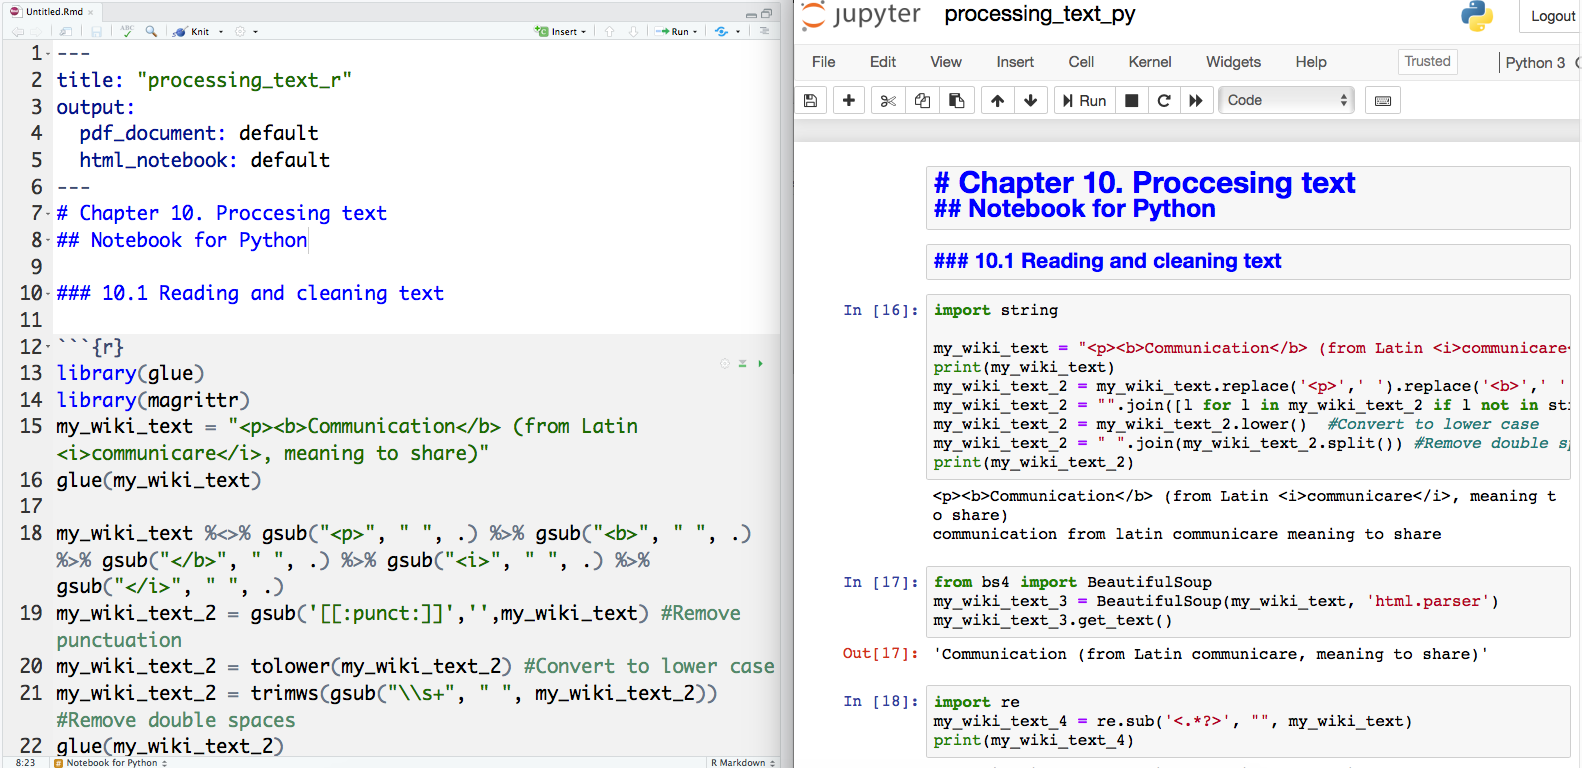
\includegraphics[width=0.9\linewidth]{figures/ch04_notebooks}
\caption{Markdown (left) and Jupyter (right) Notebooks}
\label{fig:notebooks}
\end{figure}

So far you have seen many of the possibilities that the world of code offers you from a technical and collaboration perspective. We will come back to ethical and normative considerations throughout the book, in particular in \refsec{ethicallegalpractical} and \refsec{ethics}.

\begin{figure}
\centering
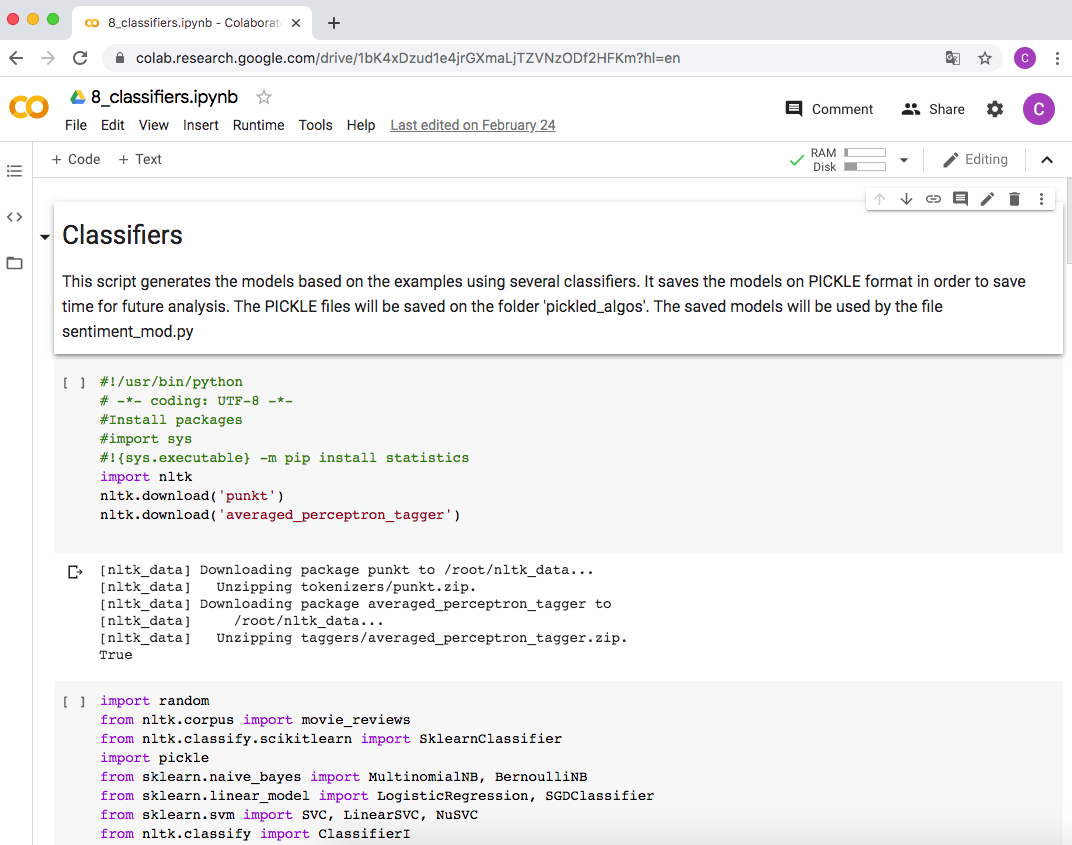
\includegraphics[width=0.9\linewidth]{figures/ch04_colab}
\caption{Jupyter notebook in Google Colab}
\label{fig:colab}
\end{figure}
